\subsection{Communication between Micro-frontends}

Micro-frontends should not depend on each other. But it is necessary to have communication between them. For example if a user adds an item to a shopping-cart in an e-commerce application, the product micro-frontend has to inform the shopping-cart micro-frontend, which item was added. To reduce the coupling between applications and development teams it is recommended to keep the communication between micro-frontends at a minimum. Before choosing a communication pattern it is important to know the type of communication. If communication between two micro-frontends or between the app shell and a micro-frontend is required, the communication can take place via the user interface. Other communication mechanisms, like the Broadcast Channel API provided by the browser, are useful for state sharing or for passing on information to multiple micro-frontends. \cite{book:2020:geers:background:micro-frontends:micro-frontends-in-action}

\bigskip

\noindent When the micro-frontends are integrated via hyperlinks, the communication can only happen via URL parameters. Single-Page-Applications usually communicate via custom events and attribute changes of the components. \cite[100]{book:2020:geers:background:micro-frontends:micro-frontends-in-action} \cite[315-316]{book:2019:farrell:background:micro-frontends:web-components-in-action} A distinction can be made between \textbf{parent-to-fragment}, \textbf{fragment-to-parent} or \textbf{fragment-to-fragment} communication, where the term fragment is equivalent to a micro-frontend and the term parent is equivalent to the app shell. \cite{book:2020:geers:background:micro-frontends:micro-frontends-in-action} This is further shown in figure \ref{fig:background:micro-frontend:communication:communication-patterns}

\ifshowImages
\begin{figure}[H]
    \centering
    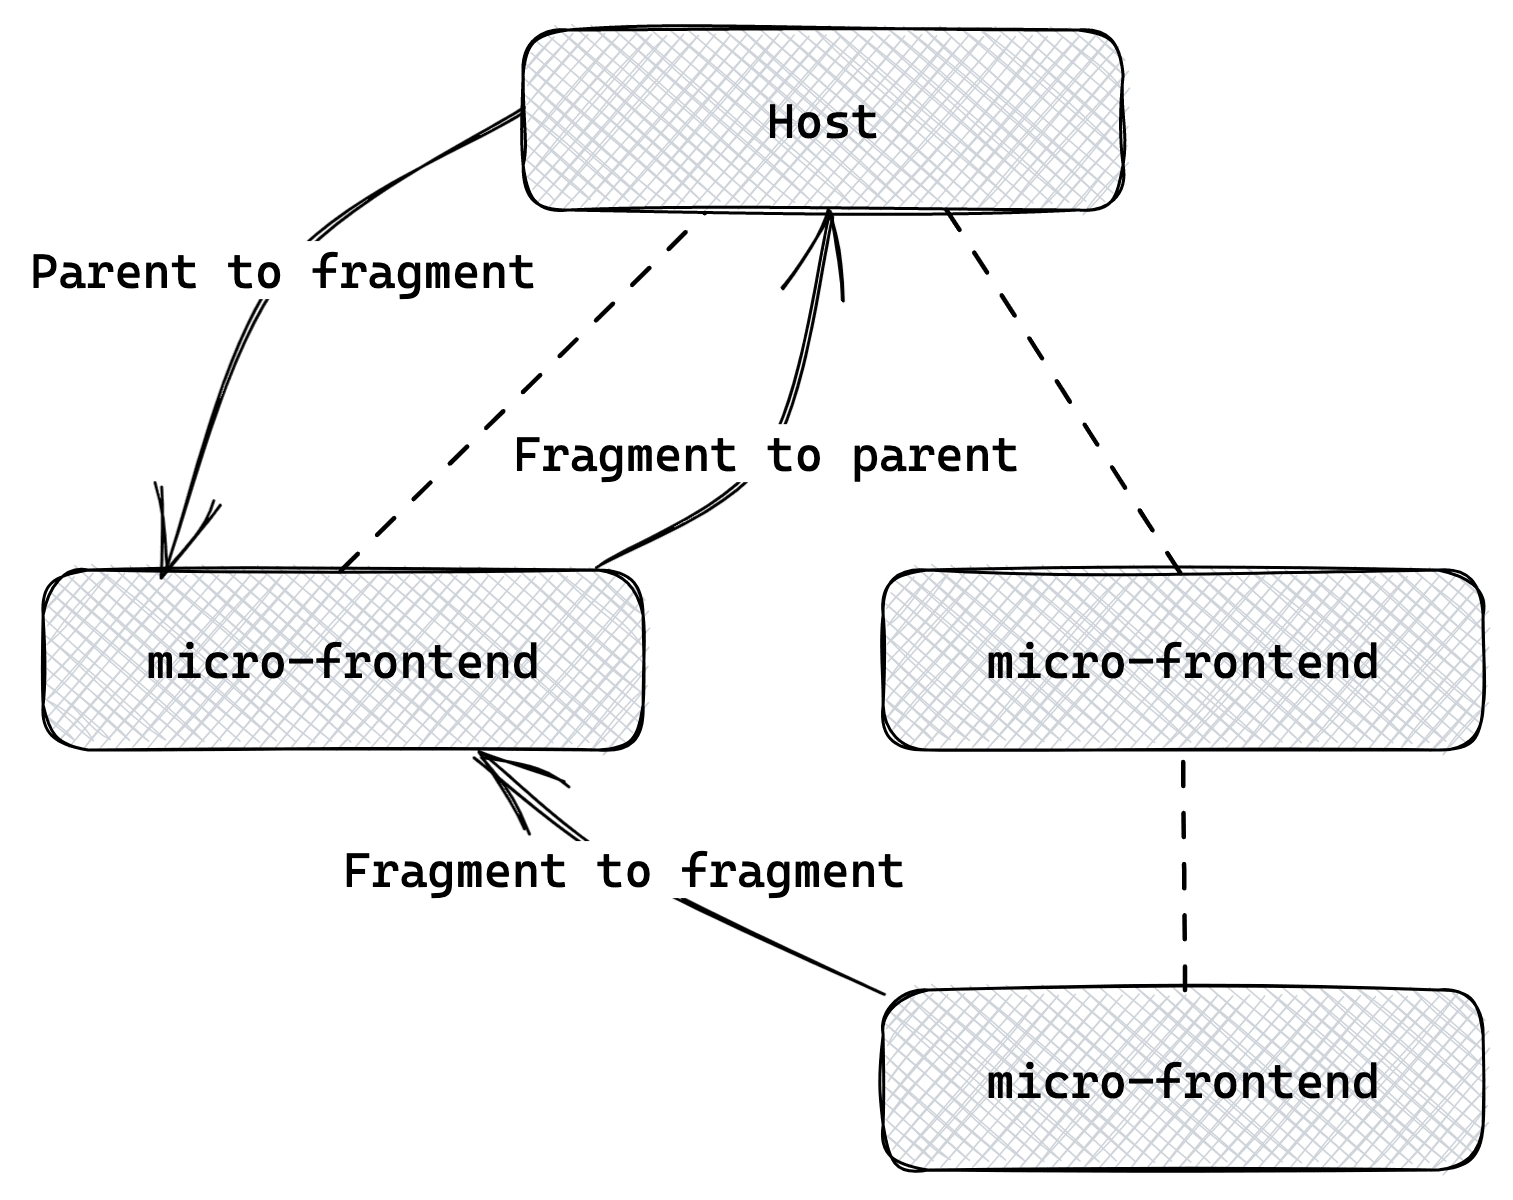
\includegraphics[width=0.5\linewidth]{images/background/communication/communication-patterns.png}
    \caption{Different forms of communication in micro-frontend architectures (Adapted from \cite[100]{book:2020:geers:background:micro-frontends:micro-frontends-in-action})}\label{fig:background:micro-frontend:communication:communication-patterns}
\end{figure}
\fi

\bigskip

\noindent Parent-to-fragment communication can happen via attribute changes when using Web Components. \cite[58-59]{book:2019:farrell:background:micro-frontends:web-components-in-action} To pass data from a micro-frontend to the app shell, custom-events can be used. \cite[315]{book:2019:farrell:background:micro-frontends:web-components-in-action}, where the micro-frontend emits an event, that the app shell is subscribed to. \cite{book:2020:geers:background:micro-frontends:micro-frontends-in-action}

\bigskip

\noindent Fragment-to-fragment communication is required when two micro-frontends should communicate with each other. The changes of one micro-frontend should have an effect on the other micro-frontend. This form of communication can be implemented in three ways: \cite[107-108]{book:2020:geers:background:micro-frontends:micro-frontends-in-action}

\begin{itemize}
    \item \textbf{Direct communication}: This is the most direct form of communication. One micro-frontend changes the attributes of its HTML elements with JavaScript. This approach is not recommended, because it introduces high coupling between two micro-frontends. One micro-frontends needs to know implementation details of the other micro-frontend. This makes it difficult to change the implementation of one micro-frontend without breaking the other micro-frontend. And this breaks one characteristics of micro-frontends, which are independent and autonomous development and deployment.
    \item \textbf{Orchestration via a parent}: When using this approach, the app shell is responsible for the communication between micro-frontends. One micro-frontend emits an event, which is intercepted by the app-shell. The app-shell sends the event to the target micro-frontend. This approach allows the micro-frontends to be completely decoupled, but changes have to be adapted by every micro-frontend.
    \item \textbf{Event-Bus/broadcasting}: Instead of a direct communication between micro-frontends or an indirect communication via the app-shell, a micro-frontend can publish an event on a central event-bus. The other micro-frontends can subscribe to the event and react to it. This is described as publish/subscribe mechanism. This drastically reduces the coupling between micro-frontends. No micro-frontend needs any information about the other micro-frontends, which allows perfect parallel development.
\end{itemize}
